 	\documentclass[10pt,letterpaper]{report}
\usepackage[utf8]{inputenc}
\usepackage{amsmath}
\usepackage{amsfonts}
\usepackage{amssymb}
\usepackage{graphicx}
\usepackage{subfig}
\author{Brandon Houghton}
\begin{document}
	
	Work completed:
	This period we implemented prediction of future states simultaneously learning invariants as well as prediction of the future state by using the activations of current and previous timestep to predict the states one time step into the future. This ensures the embeddings learned by the network encode information necessary to simulate the trajectory. Specifically we tested removing a specific arc from the training data to test how well the learned invariant would generalize. We hypothesized learned invariants would be more robust and could generalize even when certain elements of a trajectory were missing, however preliminary results show the learned invariant phi does not generalize well over the missing section of the trajectory. More investigation is needed to determine if generalize is possible with a particular set of hyperparameters.
	
	Following the future prediction model, we ran experiments squeezing the dimension of the data to create an auto encoder model. This allows us to further reduce the input space as 2D orbital positions have limited degrees of freedom. We see similar training performance in the auto-encoder model indicating that the reduced dimensionality of the input space does not reduce the expressiveness of the state – this is an important feature as we are seeking fundamental invariants and extra parameters can encourage overfitting.
	
	As we have developed many novel parameters within the loss function, it is prudent to perform a hyperparameter sweep in order to assess which parameters contribute the which properties of the learned invariant phi, as well as determining the robustness of our approach. We began exploring the parameter space manually and are working on a framework to automatically refine the hyper-parameter space and recoding the accuracy against a learned linear combination of known invariants. 
	
	We also delivered graphs and slides concerning our progress so far targeted for the presentation. Slides featured new graphs demonstrating the learned invariant and comparing it to a linear model of the angular momentum and the potential energy representing a learned energy function. 
	
	Further work is needed to fit this linear model during training to make informed decisions about early termination of training and to inform the hyperparameter optimization. That will allow us to test new formulations while getting immediate feedback that the learned function is recovering important physically defined invariants.
	
	



\begin{figure}
	\centering
	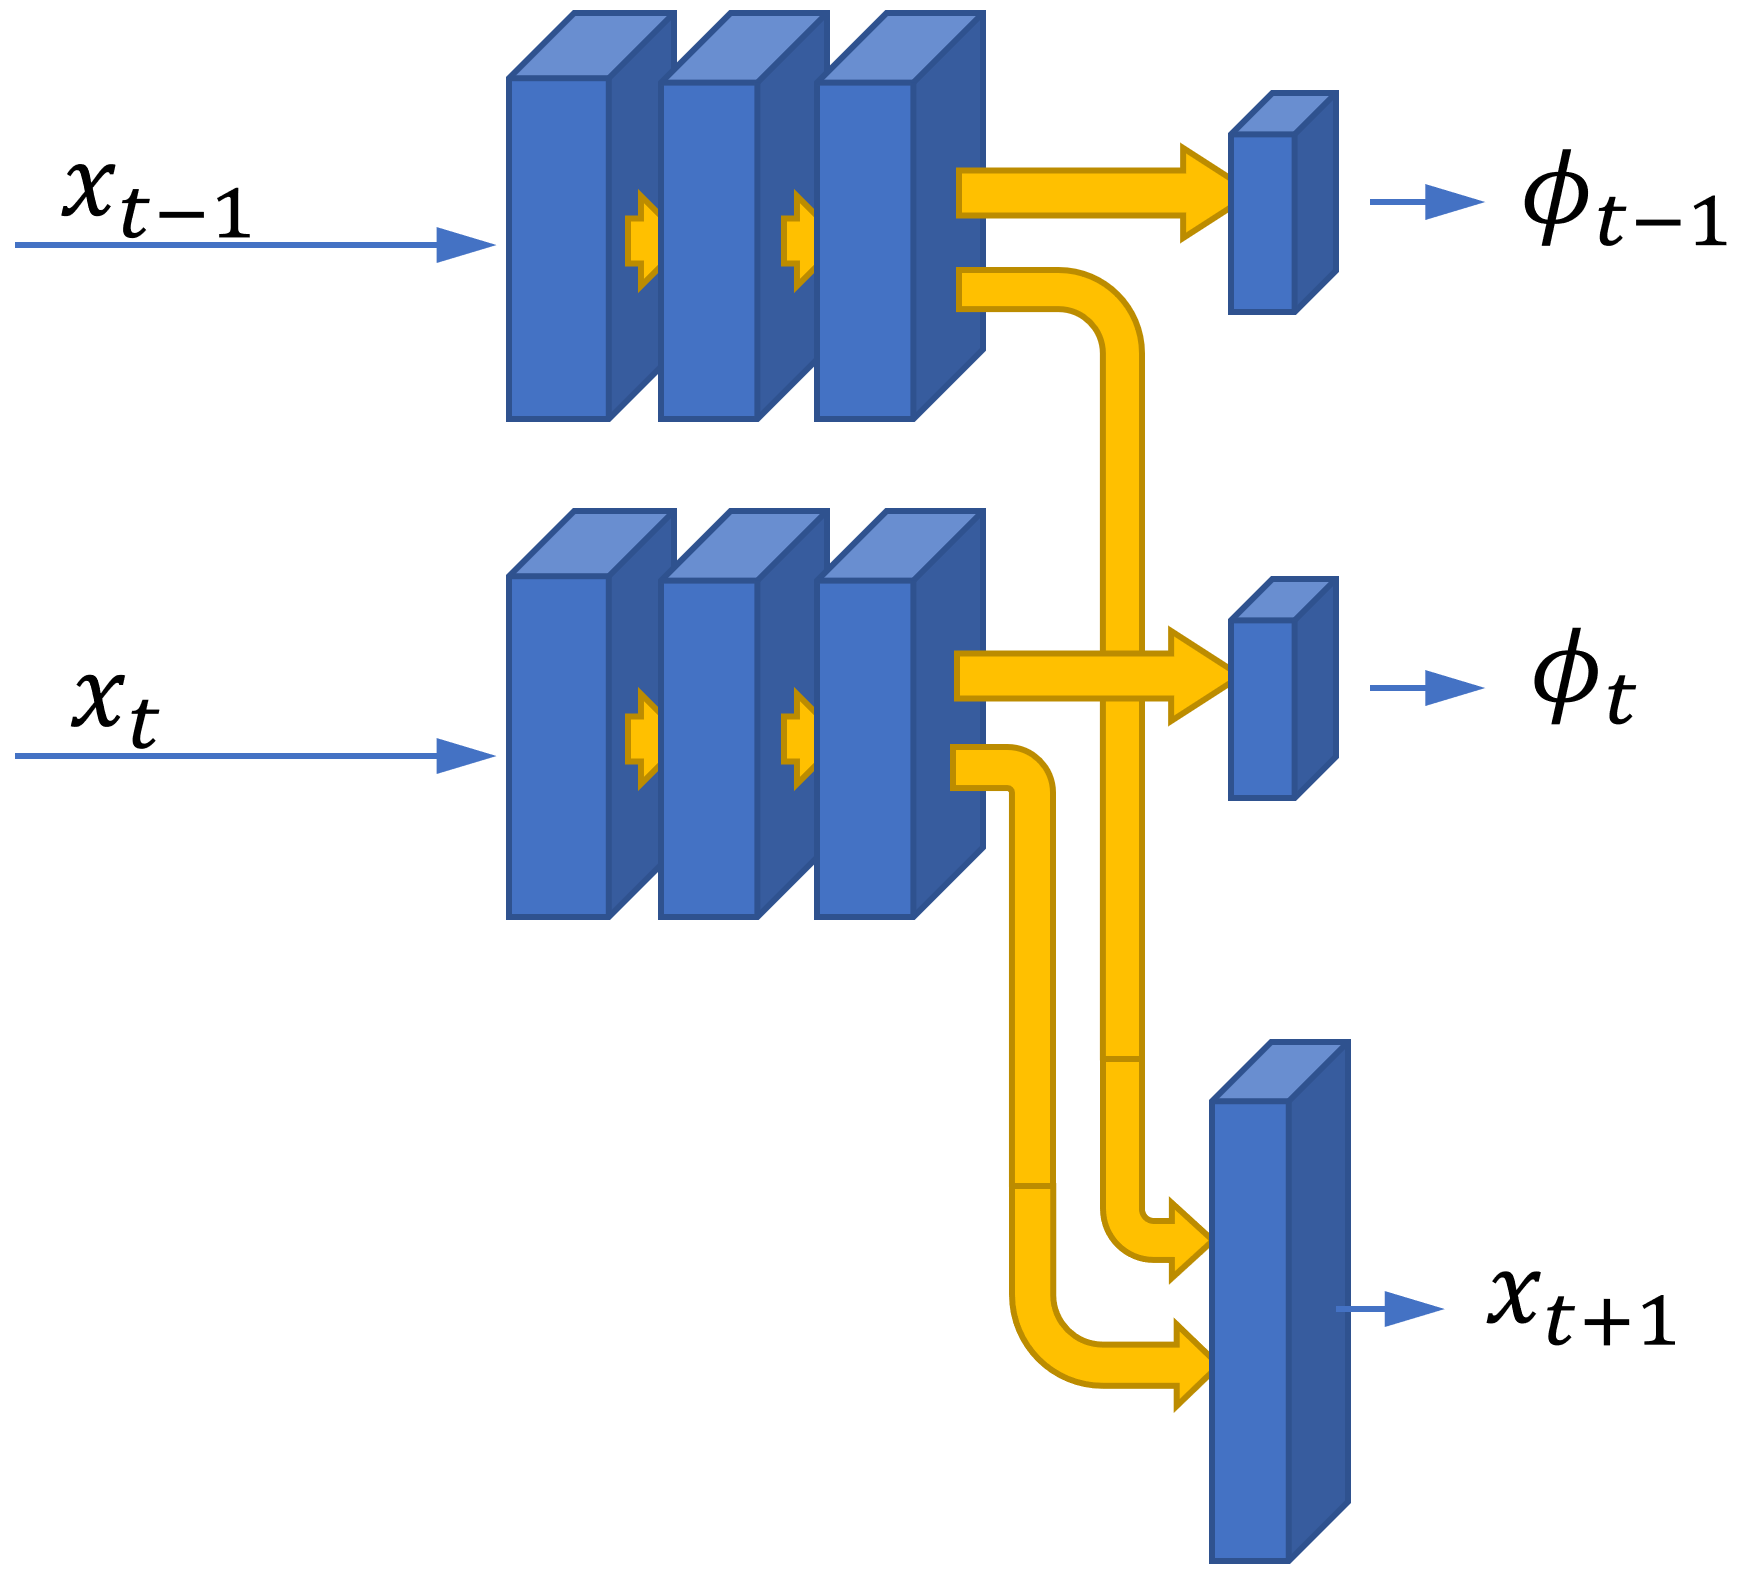
\includegraphics[width=0.7\linewidth]{./images/predNetwork}
	\caption{Network for prediction of future state - in the auto-encoder model the second layer is reduced to feature only two outputs}
	\label{fig:prednetwork}
\end{figure}



\begin{figure}%
	\centering
	\subfloat[No prediction loss]{{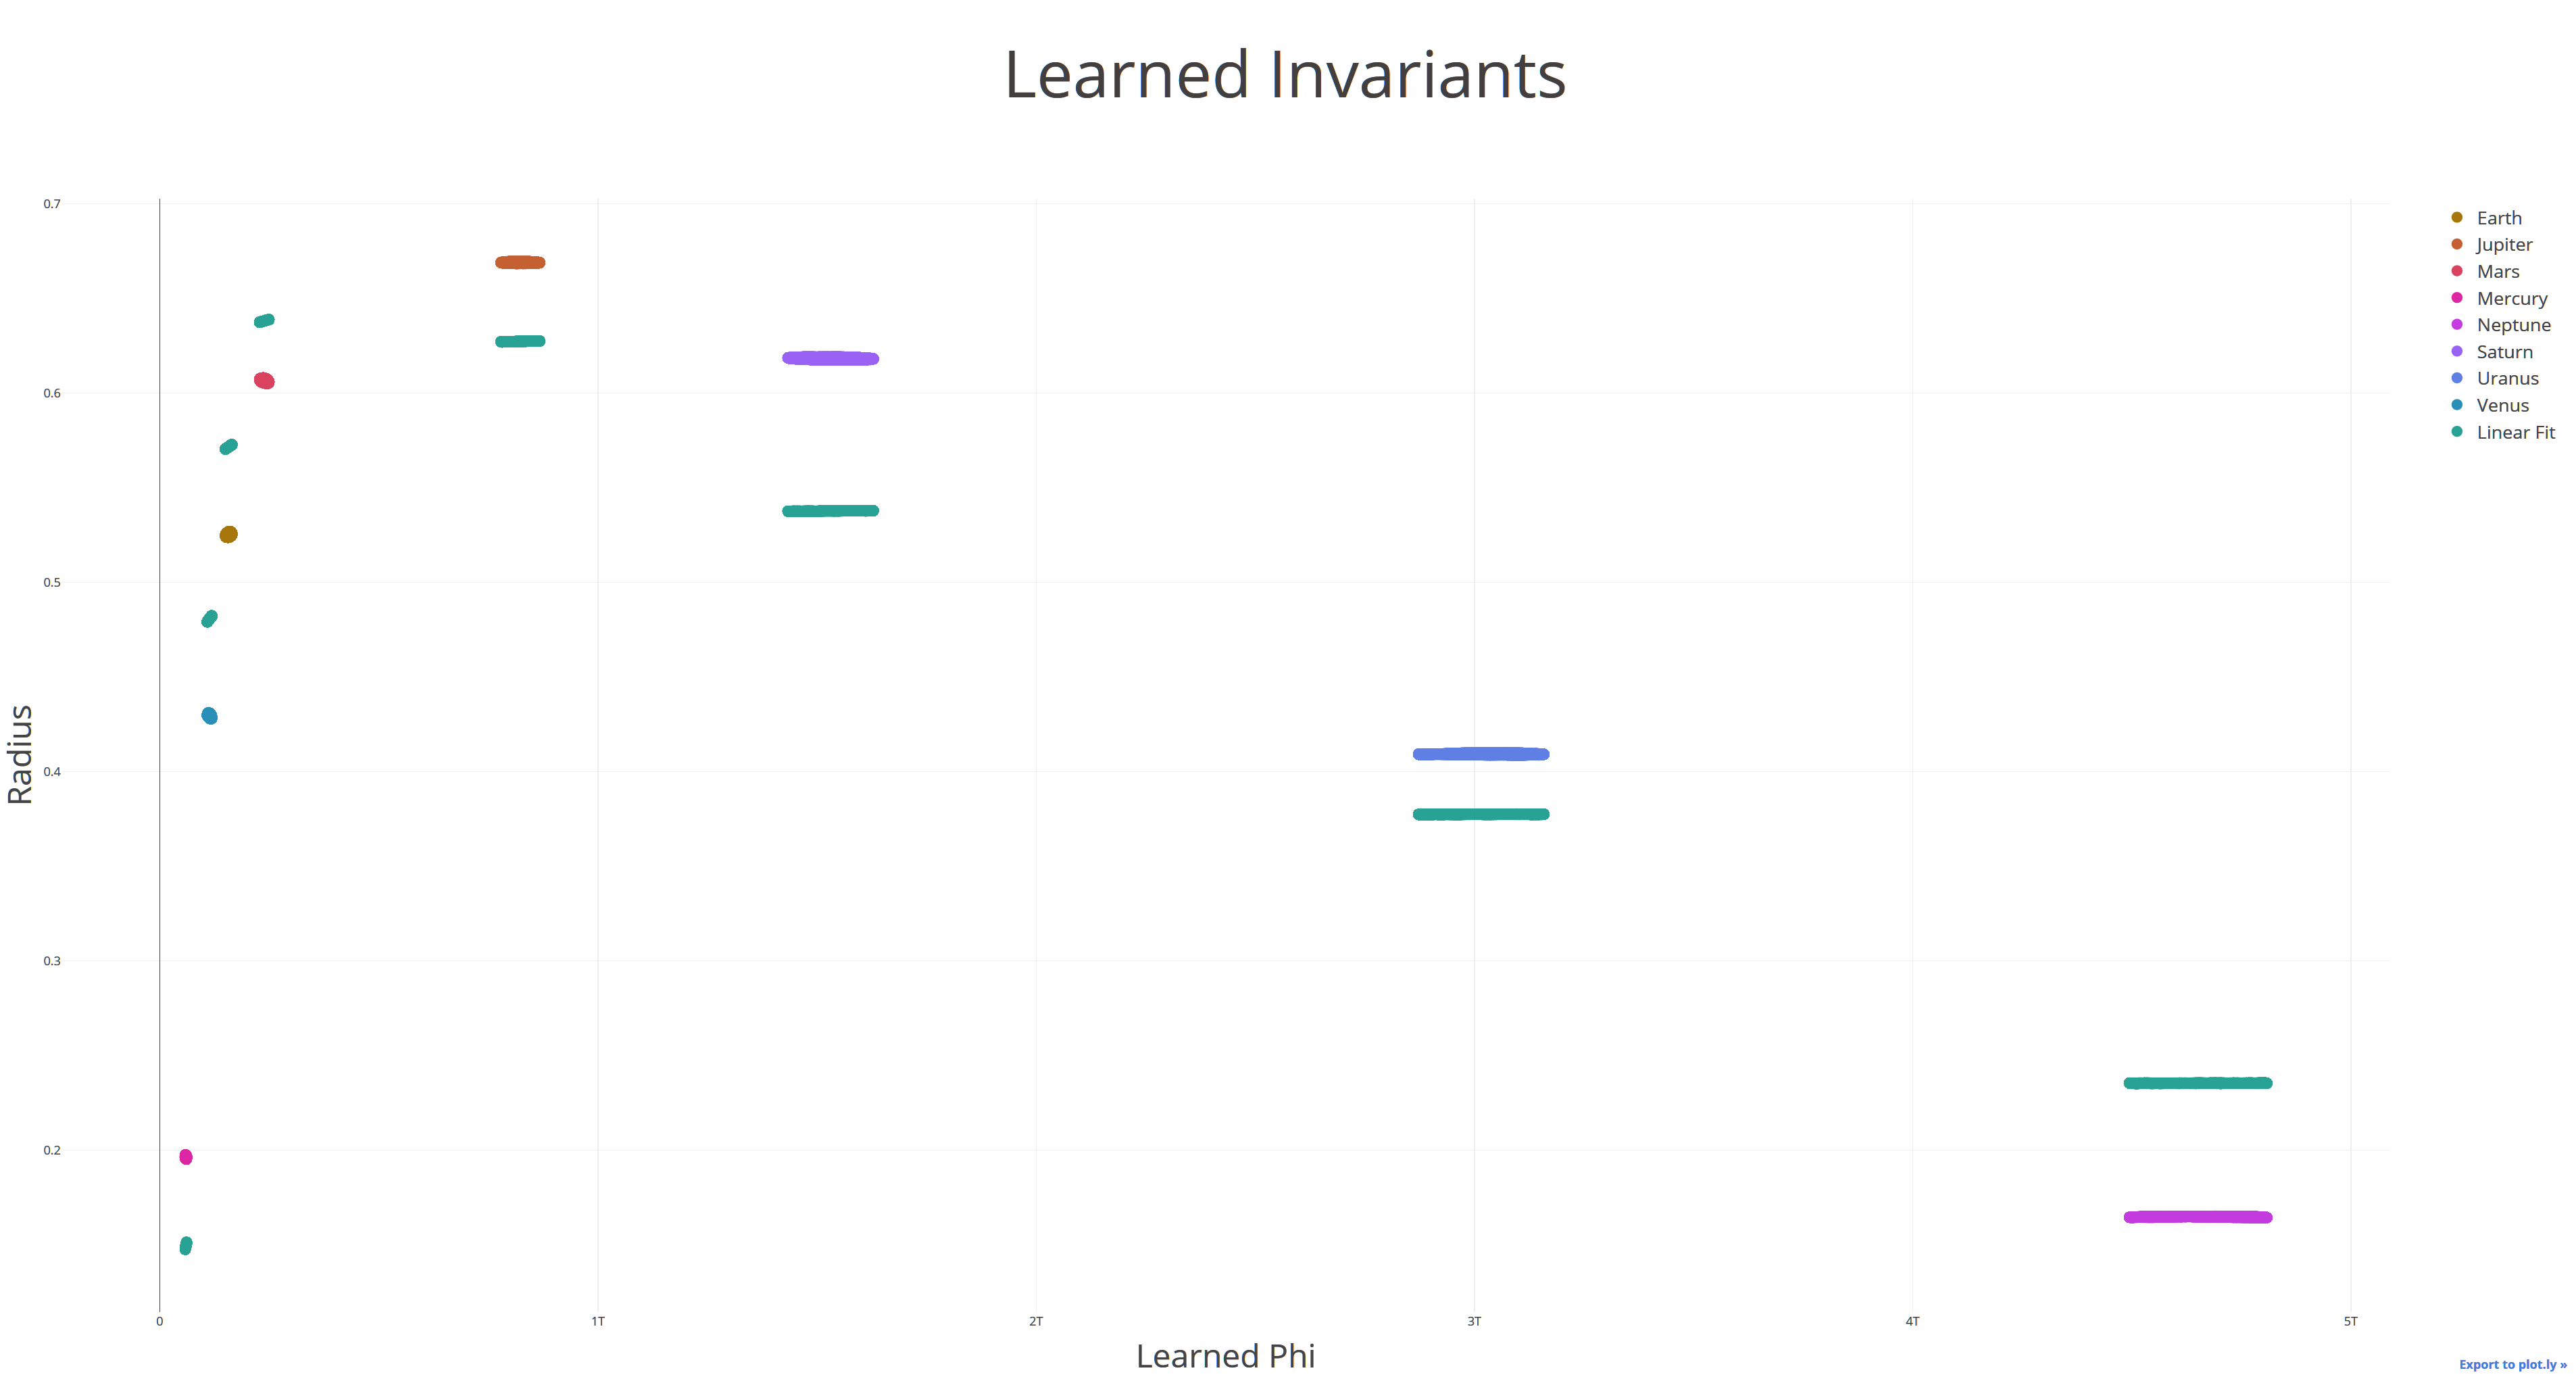
\includegraphics[width=1\linewidth]{./images/normal_fit_plot.PNG}}}
	\caption{Prediction of phi using a linear model of known invariants - linear model shows simmilar shape but some additional terms exist in the learned function phi. By searching the hyperparameter space we hope to find a network that recovers a phi that is perfectly modeled by this linear formulation }
	\label{fig:overfit}
\end{figure}




\end{document}